\documentclass[letterpaper,twocolumn,10pt,review,anonymous]{article}

\usepackage{usenix}
%%
%% \BibTeX command to typeset BibTeX logo in the docs
\AtBeginDocument{%
  \providecommand\BibTeX{{%
    Bib\TeX}}}

\newcommand{\outline}[1]{\mytodocyan{[outline: #1]}}
\newcommand{\mytodocyan}[1]{\textcolor{cyan}{\ding{46}~{\sf}~#1}}

\newcommand{\hy}[1]{\mytodopink{[hy: #1]}}
\newcommand{\mytodopink}[1]{\textcolor{violet}{\ding{46}~{\sf}~#1}}

\newcommand{\fw}[1]{\mytodored{[fw: #1]}}
\newcommand{\mytodored}[1]{\textcolor{red}{\ding{46}~{\sf}~#1}}

\newcommand{\yj}[1]{\mytodopink{[yj: #1]}}

\definecolor{wsorange}{RGB}{245,166,115}
\newcommand{\mytodoblue}[1]{\textcolor{blue}{\ding{46}~{\sf}~#1}}
\newcommand{\mytodoorange}[1]{\textcolor{wsorange}{\ding{46}~{\sf}~#1}}
\newcommand{\ws}[1]{\mytodoorange{[ws: #1]}}
\newcommand{\zl}[1]{\textcolor{SeaGreen}{\ding{46}~[zl: #1]}}
\newcommand{\fixme}[1]{{\color{blue}{#1}}} 
\newcommand{\sw}[1]{{\color{blue}{\small SW: #1}}} 

\newcommand{\bug}[1]{\noindent\textit{#1}}

\newcommand{\parh}[1]{\noindent\textbf{#1}}
\newcommand{\parhs}[1]{\noindent\underline{\textit{#1}}}
\usepackage{threeparttable}
\usepackage{xspace}
\usepackage{amsmath,amsfonts}
\usepackage{graphicx}
\usepackage{textcomp}
\usepackage{xcolor}
\usepackage{threeparttable}
\usepackage{colortbl}
\usepackage{graphicx}
\usepackage{listings}
\usepackage{color}
%\usepackage[dvipsnames]{xcolor}
\usepackage{array}
\usepackage{float}
\usepackage{graphicx}
\usepackage{multirow}
\usepackage{colortbl}
\usepackage[ruled,linesnumbered,boxed]{algorithm2e}
\usepackage{algpseudocode}
\usepackage{pifont}
\usepackage{enumitem}
\usepackage{balance}
\usepackage{xurl}
\usepackage{hyperref}
\usepackage[T1]{fontenc}
\usepackage[utf8]{inputenc}
\usepackage{caption}
\usepackage{booktabs}
\usepackage{tabularx}
\usepackage{diagbox}
\usepackage{amsmath}
\usepackage{listings}
\usepackage{makecell}
\usepackage{verbatim}
\usepackage{acronym}
\usepackage[super]{nth}
\usepackage{tikz}
\usepackage{amsmath}
\usepackage{filecontents}
\usepackage[misc]{ifsym}
\usepackage{grffile}
\usepackage{tikz,pgf}
\usepackage{amsthm}
\usepackage[most]{tcolorbox}
\usepackage{enumitem}
\usepackage{trimclip}

\newtheorem*{mydef}{Definition}
\newtheorem*{mycol}{Corollary}

\usetikzlibrary{calc}
\usetikzlibrary{positioning, fit, backgrounds, arrows.meta}
\makeatletter
\def\mfontsize{\f@size}
\newcommand*\circled[1]{\tikz[baseline=(char.base)]{
		\node[shape=circle,draw,inner sep=0pt] (char) {#1};}}


\newcommand{\F}{Fig.}
\newcommand{\E}{Eq.}
%\renewcommand{\F}{Figure}
\newcommand{\T}{Table}
%\renewcommand{\S}{Section}
\renewcommand{\S}{Sec.}
\newcommand{\A}{Alg.}
\newcommand{\highlight}[1]{{\color{red}\textbf{#1}}}



\usepackage{xcolor}

%\usepackage{minted}  % Commented out: not used and requires pygmentize

\definecolor{codegreen}{rgb}{0,0.6,0}
\definecolor{codegray}{rgb}{0.5,0.5,0.5}
\definecolor{codepurple}{rgb}{0.58,0,0.82}
\definecolor{backcolour}{rgb}{0.95,0.95,0.92}
\definecolor{cadmiumgreen}{rgb}{0.0, 0.42, 0.24}
\lstdefinestyle{mystyle}{
	%keywordstyle=\color{cadmiumgreen},
	escapeinside={(*@}{@*)},
	backgroundcolor=\color{backcolour},   
	commentstyle=\color{codegreen},
	keywordstyle=\color{magenta},
	numberstyle=\tiny\color{codegray},
	stringstyle=\color{codepurple},
	frame=shadowbox,
	basicstyle=\ttfamily\footnotesize,
	breakatwhitespace=false,         
	breaklines=true,                 
	captionpos=b,                    
	keepspaces=true,                 
	numbers=left,                    
	numbersep=5pt,                  
	showspaces=false,                
	showstringspaces=false,
	showtabs=false,                  
	tabsize=2,
}

\lstdefinestyle{gdb}
{
	backgroundcolor=\color{backcolour},
	%backgroundcolor=\color{black},
	%keywordstyle=\color{cadmiumgreen},
	keywordstyle=\color{magenta},
	escapeinside={(*@}{@*)},
	basicstyle=\scriptsize\color{black}\ttfamily,
	frame=shadowbox
}

%\renewcommand{\baselinestretch}{0.986}


\usepackage{subcaption}
\begin{document}

\title{GPU-Fuzz: A Constraint-Guided Fuzzer for Finding Memory Errors in GPU-Accelerated Deep Learning Frameworks}

\author{NAME}


\maketitle
\begin{abstract}
GPU memory errors represent an imminent and important threat to the reliability of deep learning (DL) frameworks, leading to system crashes and silent data corruption. However, discovering these bugs is challenging because existing fuzzers for DL systems focus on the neural network structure to find compiler logic errors. While effective for their purpose, they do not systematically explore the intricate operator parameter space where conditions that trigger low-level GPU memory errors lie. This paper introduces \textsc{Gpu-Fuzz}, a fuzzer specifically engineered to address this gap. Unlike structure-oriented fuzzers, \textsc{Gpu-Fuzz} models the complex relationships between operator parameters as formal constraints. It then uses a constraint solver to generate test cases that probe boundary conditions prone to memory errors in GPU kernels. By applying \textsc{Gpu-Fuzz} to major frameworks like PyTorch and TensorFlow, we discovered 14 previously unknown bugs, the majority of which are critical memory-related errors. Our work demonstrates that focusing on the operator parameter space is a highly effective and complementary approach for securing the foundational layers of modern DL systems.
\end{abstract}

\section{Introduction}
\label{sec:intro}

The security of GPU computations within deep learning (DL) frameworks like PyTorch and TensorFlow is critical. An imminent and important threat in this domain is the prevalence of GPU memory errors, a severe and insidious class of vulnerabilities stemming from the low-level CUDA kernels that implement DL operators. These errors, such as out-of-bounds access or misaligned memory addressing, can lead not only to system crashes but also to silent data corruption, posing a significant threat to the reliability and security of AI applications.

However, discovering these memory-related bugs remains a profound challenge. Existing fuzzers for DL systems are primarily designed to find logical bugs in the compiler stack by generating entire neural networks. This network-level focus, while effective for compiler testing, is ill-suited for uncovering memory errors that lie deep within the parameter space of individual operators.

Our key insight is that uncovering GPU memory errors requires a shift in focus from the network structure to the operator parameters and memory layout. The precise combination of tensor shapes, data types, strides, and other parameters dictates the memory access patterns within a CUDA kernel. To effectively find memory bugs, a fuzzer must be able to reason about these intricate constraints and generate inputs that specifically stress the memory management logic.

To this end, we designed and implemented \textsc{Gpu-Fuzz}, a novel fuzzer specifically engineered to address the threat of GPU memory errors. Unlike structure-oriented fuzzers, \textsc{Gpu-Fuzz} focuses on the operator level. It translates the complex semantic and memory-related rules of DL operators into formal constraints, which are then solved to generate precise inputs that probe memory-related boundary conditions. This constraint-guided approach enables \textsc{Gpu-Fuzz} to bypass the frameworks' frontend validation and directly stress-test the low-level CUDA kernels for memory safety.

The main contributions of this paper are as follows:
\begin{itemize}
    \item We propose a new fuzzing methodology that targets GPU memory errors by systematically exploring the operator parameter space, a dimension orthogonal to existing network structure fuzzers.
    \item We design and implement \textsc{Gpu-Fuzz}, a system that embodies this methodology by leveraging constraint solving to automatically generate test cases that probe memory-related boundary conditions in low-level CUDA kernels.
    \item We demonstrate the effectiveness of \textsc{Gpu-Fuzz} by discovering 14 previously unknown bugs, the majority being severe memory errors, in major DL frameworks and provide public minimal reproducers to benefit the community.
\end{itemize}

\section{Preliminary and Motivation}
\label{sec:bg}

\subsection{Background}
GPU kernels, typically written in CUDA, are susceptible to various memory errors. Our work focuses on critical bugs such as illegal memory accesses (out-of-bounds reads/writes), misaligned memory accesses, and race conditions, which can lead to silent data corruption or system crashes.

To detect these low-level errors, we use NVIDIA's \texttt{compute-sanitizer} as our primary test oracle. It is a powerful runtime tool that instruments GPU code to check for memory safety violations. When an error is detected, it terminates the application and provides a detailed report, enabling us to identify bugs that do not cause crashes at the API level.

\subsection{Motivation}

Our research is motivated by a critical gap in existing fuzzing methodologies for deep learning systems.

\parh{Compiler-Centric Focus of Existing Fuzzers.} State-of-the-art fuzzers for DL frameworks, such as NNSmith, have primarily focused on testing the compiler stack. Their methodology involves generating structurally valid neural networks to uncover logical inconsistencies and wrong-computation bugs that arise during graph-level optimizations. While highly effective for discovering compiler bugs, this network-level perspective is not designed to probe for low-level vulnerabilities within the CUDA kernels of individual operators.

\parh{The Operator-Level Blind Spot for Memory Errors.} GPU memory errors—such as out-of-bounds access or misaligned addressing—are not typically triggered by the high-level network architecture. Instead, they are instigated by specific, often boundary-value, combinations of an operator's parameters, including tensor shapes, data types, strides, and padding. These parameters directly dictate the memory access patterns within a CUDA kernel. Consequently, fuzzers that operate at the network structure level have a fundamental blind spot: they do not systematically explore the intricate parameter space of individual operators where these critical memory-related bugs reside.

These observations reveal the need for a paradigm shift in fuzzing for GPU security. We require a fuzzer that moves beyond the network structure to focus directly on the operator level. This motivates the design of GPU-Fuzz, a system engineered to systematically explore the operator parameter space to uncover memory safety violations in low-level CUDA kernels.

\section{System Design}
\label{sec:design}

This section details the architecture of GPU-Fuzz. As illustrated in Figure~\ref{fig:arch}, the system is designed around a data flow that seamlessly connects constraint-based test case generation with cross-framework execution, monitoring, and log-based reproduction.

\begin{figure}[htbp]
	\centering
	\resizebox{0.7\linewidth}{!}{
	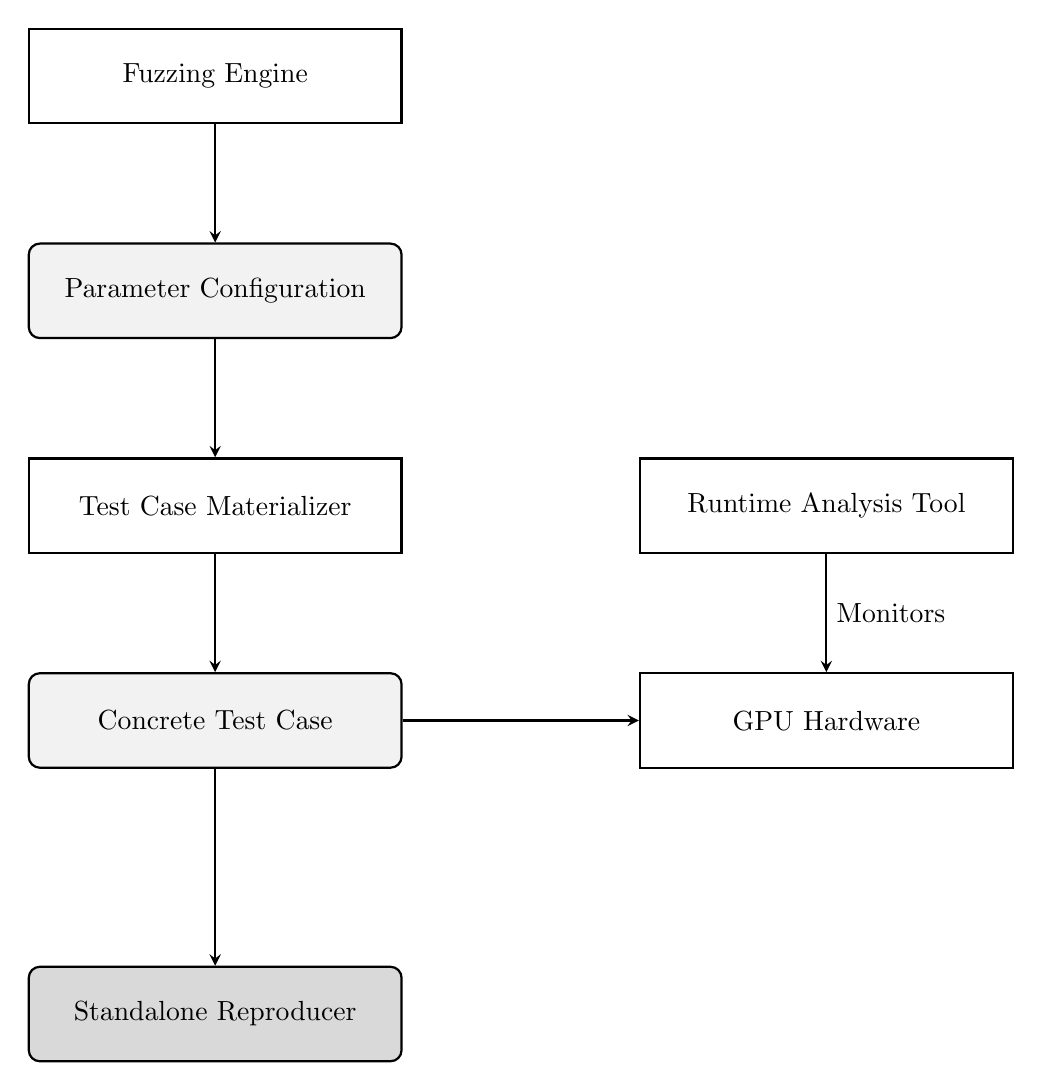
\begin{tikzpicture}[
		node distance=1.5cm,
		% Styles
		box/.style={rectangle, draw=black, thick, fill=white, minimum height=1.2cm, text width=4.5cm, text centered},
		artifact/.style={box, fill=black!5, rounded corners},
		final_artifact/.style={artifact, fill=black!15},
		arrow/.style={->, >=stealth, thick}
	]

	% --- Main linear flow ---
	\node[box] (fuzz_engine) {Fuzzing Engine};
	\node[artifact] (param_config) [below=of fuzz_engine] {Parameter Configuration};
	\node[box] (materializer) [below=of param_config] {Test Case Materializer};
	\node[artifact] (concrete_test_case) [below=of materializer] {Concrete Test Case};

	% --- Execution side-branch ---
	\node[box] (gpu) [right=3cm of concrete_test_case] {GPU Hardware};
	\node[box] (oracle) [above=of gpu] {Runtime Analysis Tool};

	% --- Final output ---
	\node[final_artifact] (reproducer) [below=2.5cm of concrete_test_case] {Standalone Reproducer};

	% --- ARROWS ---
	% Main data flow
	\draw[arrow] (fuzz_engine) -- (param_config);
	\draw[arrow] (param_config) -- (materializer);
	\draw[arrow] (materializer) -- (concrete_test_case);

	% Execution flow
	\draw[arrow] (concrete_test_case) -- (gpu);
	\draw[arrow] (oracle) -- (gpu) node[midway, right] {Monitors};
	
	% Connection to reproducer
	\draw[arrow] (concrete_test_case) -- (reproducer);

	\end{tikzpicture}
	} % end of resizebox
	\caption{The architecture of the GPU-Fuzz system.}
	\label{fig:arch}
\end{figure}

\subsection{Constraint Library and Operator Modeling}
The foundation of GPU-Fuzz is its ability to generate semantically valid inputs. This is achieved through a Constraint Library that models the operational semantics of deep learning operators. For each target operator (e.g., convolution, pooling, matrix multiplication), we define a set of constraints that capture the legitimate relationships between its parameters, such as tensor shapes, data types, kernel sizes, strides, and padding. These constraints create a framework-agnostic representation of the operator's contract. This approach ensures that any test case generated is, by construction, guaranteed to pass the framework's initial validation checks.

\subsection{Constraint-based Test Case Generation}
The core of the fuzzing loop resides in the test case generator. The process begins by randomly selecting an operator template from the Constraint Library. The generator then populates the template with randomized, but plausible, target dimensions and parameters. These parameters, along with the operator's formal constraints, are passed to a constraint solver. The solver's task is to find a concrete assignment of values that satisfies all constraints. The result is a complete set of valid parameters (e.g., \texttt{input\_shape}, \texttt{kernel\_size}, \texttt{stride}) and the corresponding output tensor shape, which together form a framework-agnostic parameter configuration.

For instance, consider a 2D convolution (\texttt{Conv2D}). The relationship between input height ($H_{in}$), output height ($H_{out}$), padding ($P$), kernel ($K$), dilation ($D$), and stride ($S$) is governed by the equation: $H_{out} = \lfloor (H_{in} + 2P - D \cdot (K - 1) - 1) / S \rfloor + 1$. Furthermore, for grouped convolutions, the number of input and output channels must both be divisible by the `groups` parameter. Our fuzzer translates these rules into a formal constraint system. It might generate a plausible $H_{in}$ and then task the solver with finding a consistent set of values for the remaining parameters that satisfy all interdependent constraints. This ensures the generated parameters are holistically consistent, a prerequisite for bypassing framework validation and testing the underlying kernel.

\subsection{Cross-Framework Execution and Monitoring}
Once a set of valid parameters is generated, this parameter configuration is materialized into an executable script for a target framework (PyTorch, TensorFlow, or PaddlePaddle). This script creates the necessary tensors, populates them with random data, and invokes the operator on the GPU.

The execution is monitored by NVIDIA's \texttt{compute-sanitizer}. This tool can detect a wide range of GPU-level errors, such as out-of-bounds memory accesses and race conditions, that would not typically cause a visible crash at the Python API level. When a violation is detected, \texttt{compute-sanitizer} terminates the process and generates a detailed report, which serves as our primary bug oracle.

\subsection{Bug Reproducibility}
To facilitate the validation and debugging of discovered vulnerabilities, \textsc{Gpu-Fuzz} systematically records the conditions that trigger each failure. This record encapsulates the target operator and framework, the specific input parameters (e.g., kernel size, stride), the shapes of all input tensors, and the random seed used for data generation. The raw input tensors are also preserved. This collection of artifacts provides a self-contained and deterministic reproducer for each bug, significantly simplifying the process of verification and root cause analysis for developers.
\section{Implementation}
\label{sec:impl}
This section details the implementation of the system design described in Section~\ref{sec:design}. Our system is developed in Python and comprises 2,628 lines of code.
    
We implemented a library where each operator is represented as a distinct class to realize the operator modeling and constraint-based test case generation concepts described in Section~\ref{sec:design}. This modeling approach was applied to 13 operators (\T~\ref{tab:operators}), chosen for their prevalence in deep learning models and their complex, error-prone memory access patterns.

The translation process (Section~\ref{sec:execution}) is implemented to translate the generated parameter values into framework-specific API calls. When compute-sanitizer~\cite{nvidia2023compsan} detects an error during execution, the system automatically archives the execution logs to ensure reproducibility.

\begin{table}[t]
    \centering
    \caption{Supported Operators in \textsc{GPU-Fuzz}}
    \label{tab:operators}
    \footnotesize
    \begin{tabular}{@{}lp{5.0cm}@{}}
    \toprule
    \textbf{Operator Family} & \textbf{Specific Operators} \\
    \midrule
    Convolution & \makecell[l]{Conv (1d, 2d, 3d), ConvTranspose (1d, 2d, 3d)} \\
    \midrule
    Pooling & \makecell[l]{MaxPool (1d, 2d, 3d), AvgPool (1d, 2d, 3d), \\ FractionalMaxPool (2d, 3d), LPPool (1d, 2d, 3d), \\ AdaptiveAvgPool (1d, 2d, 3d),\\ AdaptiveMaxPool (1d, 2d, 3d)} \\
    \midrule
    Padding & \makecell[l]{ReflectionPad (1d, 2d, 3d),\\ ReplicationPad (1d, 2d, 3d),\\ ZeroPad (1d, 2d, 3d), ConstantPad (1d, 2d, 3d),\\ CircularPad (1d, 2d, 3d)} \\
    \midrule
    Element-Wise Unary & \makecell[l]{Activation: ELU, ReLU, GELU, Sigmoid, Tanh, ...\\ Arithmetic: abs, sin, cos, sqrt, exp, log, ...} \\
    \midrule
    Element-Wise Binary & \makecell[l]{add, sub, mul, div, pow, remainder,\\ logaddexp, atan2, ...} \\
    \midrule
    Matrix Ops & MatMul, BMM \\
    \midrule
    Concat & cat, concat \\
    \bottomrule
    \end{tabular}
    \end{table}
    \vspace{-0.4em}
\section{Evaluation}
\label{sec:eval}

In this section, we evaluate the effectiveness and efficiency of \textsc{GPU-Fuzz}. We aim to answer the following research questions (RQs):
\begin{itemize}[leftmargin=1em]
    \item \textbf{RQ1:} How effective is \textsc{GPU-Fuzz} in uncovering real-world bugs in major deep learning frameworks?
    \item \textbf{RQ2:} How does \textsc{GPU-Fuzz} compare with state-of-the-art DL fuzzers in terms of test case generation and bug discovery, particularly for GPU memory errors?
\end{itemize}

\subsection{Experimental Setup}
\label{sec:setup}
All experiments were conducted on a server with the configuration detailed in \T~\ref{tbl:setup}. We established isolated Conda environments for each of the three target frameworks (PyTorch, TensorFlow, and PaddlePaddle) to manage their specific dependencies. The core hardware, operating system, and NVIDIA driver were consistent across all tests.

\begin{table}[h!]
\centering
\caption{Experimental Environment Configuration.}
\label{tbl:setup}
\footnotesize
\begin{tabular}{@{}ll@{}}
\toprule
\textbf{Component} & \textbf{Specification} \\ \midrule
\multicolumn{2}{@{}l}{\textbf{Hardware}} \\
\hspace{1em}CPU & 2 x Intel Xeon Silver 4510 \\
\hspace{1em}GPU & NVIDIA H100 PCIe \\
\midrule
\multicolumn{2}{@{}l}{\textbf{Software}} \\
\hspace{1em}Operating System & Ubuntu 24.04.2 LTS \\
\hspace{1em}NVIDIA Driver & 580.82.07 \\
\hspace{1em}CUDA Runtime & 12.8.93 \\
\hspace{1em}Python & 3.11.13 \\
\midrule
\multicolumn{2}{@{}l}{\textbf{Frameworks}} \\
\hspace{1em}PyTorch & PyTorch 2.3.1+cu121 with cuDNN 8.9.2.26 \\
\hspace{1em}TensorFlow & 2.20.0, with cuDNN 9.13.0.50 \\
\hspace{1em}PaddlePaddle & 2.6.1 \\
\bottomrule
\end{tabular}%
\end{table}

\subsection{Bug Discovery Effectiveness}

Over the course of our evaluation, \textsc{GPU-Fuzz} uncovered a total of 13 previously unknown bugs across the three frameworks. \T~\ref{tbl:bugs} presents a summary of these findings. The bugs span a range of failure modes, from low-level memory corruption to API-level exceptions. 
We identified 7 distinct memory access violations (e.g., out-of-bounds or misaligned writes). Among these, 5 were silent memory corruptions that do not trigger any API-level crash and are only detectable with specialized tools like compute-sanitizer~\cite{nvidia2023compsan}. 

\begin{table*}[htbp]
\centering
\caption{Summary of Bugs Discovered by \textsc{GPU-Fuzz}.}
\label{tbl:bugs}
\resizebox{\textwidth}{!}{%
\begin{tabular}{@{}lllllll@{}}
\toprule
\textbf{ID} & \textbf{Framework} & \textbf{Operator} & \textbf{Bug Type} & \textbf{Root Cause} & \textbf{Failure Mode} & \textbf{Status} \\ \midrule
\textbf{Bug\textsubscript{1}} & PyTorch & \texttt{conv\_transpose2d} & OOB Global Write & Incorrect grid dimension calculation & GPU-Level Exception (CUBLAS) & Confirmed \\
\textbf{Bug\textsubscript{2}} & PyTorch & \texttt{bmm\_sparse} & Misaligned Global Write & Incorrect pointer arithmetic in CUSPARSE & Silent Memory Corruption & Reported \\
\textbf{Bug\textsubscript{3}} & PyTorch & \texttt{adaptive\_avg\_pool2d} & OOB Global Write & Flawed boundary checks in CUDA kernel & Silent Memory Corruption & Confirmed \\
\textbf{Bug\textsubscript{4}} & PyTorch & \texttt{replication\_pad2d} & OOB Global Write & Incorrect grid dimension calculation & Silent Memory Corruption & Confirmed \\
\textbf{Bug\textsubscript{5}} & PyTorch & \texttt{adaptive\_max\_pool2d} & OOB Global Write & Flawed boundary checks in CUDA kernel & Silent Memory Corruption & Confirmed \\
\textbf{Bug\textsubscript{6}} & PyTorch & \texttt{conv\_transpose3d} & OOB Shared Read & Incorrect index calculation for shared memory & Silent Memory Corruption & Fixed \\
\textbf{Bug\textsubscript{7}} & PyTorch & \texttt{reflection\_pad1d} & Invalid Launch Config & Integer overflow in \texttt{torch.compile} symint logic & GPU-Level Exception (CUDA) & Confirmed \\
\textbf{Bug\textsubscript{8}} & TensorFlow & \texttt{Conv2D} & OOB Global Read & Incorrect index calculation in kernel & Silent Read / Downstream Crash & Confirmed \\
\textbf{Bug\textsubscript{9}} & TensorFlow & \texttt{Conv2D} & Integer Overflow & Overflow in launch config calculation & CPU-Side Assert & Confirmed \\
\textbf{Bug\textsubscript{10}} & PaddlePaddle & \texttt{conv2d\_transpose} & Precondition Violation & Integer overflow in tensor dimension calculation & CPU-Side Assert & Confirmed \\
\textbf{Bug\textsubscript{11}} & PaddlePaddle & \texttt{conv3d\_transpose} & Illegal Instruction & Invalid parameters passed to cuDNN kernel & GPU-Level Exception (cuDNN) & Confirmed \\
\textbf{Bug\textsubscript{12}} & PaddlePaddle & \texttt{conv2d\_transpose} & Bad API Parameter & Invalid parameter combination passed to cuDNN & GPU-Level Exception (cuDNN) & Confirmed \\
\textbf{Bug\textsubscript{13}} & PaddlePaddle & \texttt{conv2d\_transpose} & Invalid Launch Config & Incorrect grid/block dimension calculation & GPU-Level Exception (CUDA) & Confirmed \\
\bottomrule
\end{tabular}
}
\end{table*}

\parh{Bug Patterns.} 
Our findings reveal important patterns across three distinct failure modes:
\begin{itemize}[leftmargin=1em]
    \item \textbf{Silent Memory Corruption:} The most critical category, where out-of-bounds or misaligned memory access occurs without causing any API-level error. These are the most insidious bugs as they can lead to silent data corruption and are only detectable with low-level memory debuggers.
    \item \textbf{GPU-Level Exceptions:} The second category, where invalid parameters or configurations cause CUDA, cuDNN, or CUBLAS libraries to return an error, which is then typically caught and reported by the framework.
    \item \textbf{CPU-Side Asserts:} The final category, where issues like integer overflows occur on the CPU during the calculation of kernel parameters, preventing the GPU launch altogether.
\end{itemize}
\noindent A common root cause across all frameworks was incorrect grid dimension calculations or flawed boundary checks, with transposed convolutions being particularly error-prone. 

\subsection{Comparative Study}
\label{sec:comparison}
To quantitatively validate our approach, we conducted a comparative study against NNSmith~\cite{liu2023nnsmith}, a state-of-the-art DL fuzzer. We conducted five independent 4-hour fuzzing runs for each tool on the same hardware targeting PyTorch, with both tools running in identical Conda environments.

\T~\ref{tbl:comparison} summarizes the results. NNSmith generated on average $19{,}063\pm 360$ test cases and uncovered $296\pm 19$ bugs. Most of its findings are numerical mismatches rather than memory-safety issues. In contrast, \textsc{GPU-Fuzz} generated on average $51{,}860\pm 1{,}559$ test cases and uncovered $106\pm 8$ real bugs excluding out-of-memory errors, including $26\pm 5$ critical memory errors and $80\pm 7$ configuration errors. These memory errors represent severe security vulnerabilities that could result in data corruption, information leakage, or system crashes.

\begin{table}[htbp]
\centering
\caption{Comparative Results}
\label{tbl:comparison}
\footnotesize
\begin{tabular}{@{}lcc@{}}
\toprule
\textbf{Metric} & \textbf{NNSmith} & \textbf{GPU-Fuzz} \\
\midrule
\textbf{Test Cases Generated} & $19{,}063\ \pm\ 360$ & $51{,}860\ \pm\ 1{,}559$ \\
\textbf{Total Bugs}\textsuperscript{*} & $296\ \pm\ 19$ & $106\ \pm\ 8$ \\
\midrule
\multicolumn{3}{@{}l}{\textbf{Bug Breakdown by Type}} \\
\hspace{1em}Memory Errors & 0 & $26\ \pm\ 5$ \\
\hspace{1em}Configuration Errors & 0 & $80\ \pm\ 7$ \\
\hspace{1em}Inconsistencies & $293\ \pm\ 19$ & 0 \\
\hspace{1em}Exceptions & $3\ \pm\ 1$ & 0 \\
\midrule
\textbf{Runtime} & \multicolumn{2}{c}{4 GPU-hours each} \\
\bottomrule
\multicolumn{3}{@{}l}{\scriptsize\textsuperscript{*}GPU-Fuzz total excludes out-of-memory errors.} \\
\multicolumn{3}{@{}l}{\scriptsize\textsuperscript{**}NNSmith and GPU-Fuzz results are mean $\pm$ std over 5 independent runs.} \\
\end{tabular}%
\end{table}

\parh{Key Findings.} 
Our analysis reveals two critical insights. First, \textsc{GPU-Fuzz} generated nearly three times more test cases than NNSmith, demonstrating the efficiency of constraint-guided parameter fuzzing in systematically exploring the operator parameter space. Second, \textsc{GPU-Fuzz} uncovered $26\pm 5$ memory errors that pose security risks, while NNSmith's findings were primarily numerical precision issues that typically do not threaten memory safety. This demonstrates that \textsc{GPU-Fuzz} addresses a blind spot in GPU memory security testing that existing DL fuzzers frequently miss. The two approaches are complementary: NNSmith excels at uncovering compiler-related bugs and numerical inconsistencies, while \textsc{GPU-Fuzz} fills the gap in GPU memory security testing at the operator parameter level.

\subsection{Case Study}
\label{sec:case_study}
To illustrate the practical utility of \textsc{GPU-Fuzz}, we present a minimal proof-of-concept (PoC) for a memory corruption bug uncovered in PyTorch's \texttt{ConvTranspose2d} operator. The PoC is shown in \F~\ref{fig:poc_code}.

\begin{figure}[htbp]
\centering
\vspace{-0.2em}
\includegraphics[width=0.9\columnwidth]{figs/code.pdf}
\vspace{-0.4em}
\caption{A minimal PoC in Python and the corresponding CUDA implementation that triggers a memory bug in PyTorch's \texttt{ConvTranspose2d}.}
\Description{A code snippet showing a minimal proof-of-concept in Python that triggers a memory corruption bug in PyTorch's ConvTranspose2d operator, along with the corresponding CUDA code demonstrating an integer overflow when calculating the total number of elements, leading to invalid memory access.}
\label{fig:poc_code}
\vspace{-0.2em}
\end{figure}

The key to triggering this bug lies in the parameter combination automatically generated by our fuzzer, particularly the extremely large stride value of $(200, 200)$ combined with input dimensions of $(10, 40000, 2)$. 
While these values are semantically valid according to PyTorch's API, they represent a corner case that is unlikely to be covered by manual tests. 
As illustrated in \F~\ref{fig:poc_code}, the root cause is an integer overflow in the C++ host code: when calculating the total number of elements for the CUDA kernel, a 64-bit integer value is cast to a 32-bit integer, which causes truncation. 
This overflowed value is then used to calculate the CUDA grid dimensions, resulting in an undersized grid that cannot cover all required memory operations. 
When the \texttt{col2im\_kernel} executes, threads calculate 64-bit indices that exceed the actual allocated buffer size, leading to out-of-bounds memory writes. 

\begin{figure}[htbp]
    \centering
    \vspace{-0.2em}
    \includegraphics[width=0.8\columnwidth]{figs/log.pdf}
    \vspace{-0.4em}
    \caption{The error message for the PoC.}
    \Description{An error log showing the error message for the proof-of-concept code in the previous figure.}
    \label{fig:poc_log}
    \vspace{-0.2em}
    \end{figure}
    
As shown in \F~\ref{fig:poc_log}, compute-sanitizer detects that a CUDA thread attempts to write to an out-of-bounds address, which is before the nearest valid allocation. 
This type of silent memory corruption is a severe bug that can lead to incorrect results or unpredictable behavior without causing an explicit Python crash, and demonstrates the ability of \textsc{GPU-Fuzz} to systematically uncover severe, hidden bugs in mature deep learning frameworks by exploring non-trivial parameter spaces.


\section{Discussion}
\label{sec:discussion}
While our results demonstrate the effectiveness of GPU-Fuzz, we acknowledge several limitations and areas for future work.

\parh{Manual Modeling Effort.} The quality of GPU-Fuzz depends on its constraint library. Our current library supports 11 operator families, but this is a subset of the hundreds of operators available. Extending coverage requires manual effort to model constraints (100-150 LoC per family). Future work could explore semi-automating constraint extraction from framework documentation to improve scalability.

\parh{Limited Oracle.} Our primary oracle, \texttt{compute-sanitizer}, excels at finding memory errors but cannot detect silent numerical correctness issues or performance regressions. Differential fuzzing against a trusted CPU implementation is a promising direction for a more comprehensive oracle.

\section{Related Work}
\label{sec:related_work}

Our work is positioned at the intersection of deep learning (DL) systems security and software testing, with a specific focus on uncovering memory-related bugs in GPU kernels.

\subsection{Fuzzing for Deep Learning Systems}
Fuzzing for DL systems primarily involves two approaches: structure-level and API-level testing.

\textbf{Structure-level fuzzers}, including NNSmith~\cite{nnsmith}, TVMFuzz~\cite{tvmfuzz}, and Lemon~\cite{lemon}, focus on generating valid neural network models to test the compiler stack. Their strength lies in identifying graph-level optimization bugs. However, their network-centric view is ill-suited for exploring the operator parameter boundaries required to trigger memory access violations in GPU kernels.

\textbf{API-level fuzzers}, such as FreeFuzz~\cite{freefuzz}, DeepREL~\cite{deeprel}, and TitanFuzz~\cite{titanfuzz}, test the API layer by generating valid sequences of function calls. While effective for detecting API-level crashes, they cannot uncover silent memory errors that occur at a lower level and are only visible via specialized tools like \texttt{compute-sanitizer}.

In contrast, \textsc{Gpu-Fuzz} is a \textbf{parameter-level fuzzer}. It complements existing work by focusing on individual operators and systematically exploring their parameter boundary conditions. This targeted approach is uniquely effective at discovering the memory safety vulnerabilities within GPU backends that other methods miss.

\subsection{GPU Security}
Other research targets the GPU software stack more directly. For example, compiler fuzzers like Cudasmith~\cite{cudasmith} generate random CUDA C programs from scratch to stress-test the CUDA compiler (\texttt{nvcc}) itself. In contrast, \textsc{Gpu-Fuzz} does not generate new CUDA code; instead, it tests the existing, domain-specific, and highly-optimized CUDA kernels that are handwritten by framework developers to implement core DL operators. Similarly, driver-level fuzzers such as GLeeFuzz~\cite{gleefuzz} and Moneta~\cite{moneta} test the GPU stack from a different angle. \textsc{Gpu-Fuzz} bridges the gap between high-level DL applications and low-level GPU execution by using the frameworks' own operators as the entry point to stress-test the underlying kernels for memory safety.

\section{Responsible Disclosure}
We have disclosed all 13 discovered bugs responsibly to the respective development teams of PyTorch~\cite{paszke2019pytorch}, TensorFlow~\cite{abadi2016tensorflow}, and PaddlePaddle~\cite{ma2019paddlepaddle} by opening detailed issue reports in their official code repositories. 
At the time of writing, several of these issues have been acknowledged by the developers. 
We are committed to collaborating with the framework maintainers to help improve the security and robustness of the deep learning ecosystem.

\section{Conclusion}
\label{sec:conclusion}
In this paper, we presented \textsc{Gpu-Fuzz}, a constraint-guided fuzzing system designed to uncover memory-related vulnerabilities in GPU-accelerated deep learning operators. We introduced a parameter-level fuzzing approach to address a critical gap left by existing structure-level fuzzers, which primarily target compiler logic errors. By modeling operator semantics as formal constraints, our system systematically generates valid test cases that probe boundary conditions prone to memory errors.

Our extensive evaluation demonstrates that this constraint-based approach is highly effective. GPU-Fuzz successfully discovered 14 unique, previously unknown bugs in major frameworks like PyTorch, TensorFlow, and PaddlePaddle, the majority of which were critical silent memory errors, undetectable at the Python API level and only discoverable through low-level monitoring.

The success of \textsc{Gpu-Fuzz} demonstrates a key takeaway for the security of modern AI systems: comprehensive testing requires a two-pronged approach. Both structure-level fuzzing to secure the compiler stack and parameter-level fuzzing to secure the underlying kernels are necessary and complementary. By making our tool and the discovered bugs publicly available, we hope to provide a valuable resource for developers and researchers working to improve the reliability and security of these foundational software systems.



\bibliographystyle{plainnat}
\bibliography{ref}

\appendix
\input{./files/appendix.tex}

\end{document}
\endinput
